

    %Abstract
    %Introduction (motivation for your work)
    %Background (literature review, or related work)
    %Methods (design and implementation)
    %Results and discussion  (include plots & figures, and detailed analysis in comparison to baseline and the literature, if applicable)
    %Conclusion

%\documentclass{article}
\documentclass[11pt,a4paper, twocolumn]{article}
%\usepackage[hyperref]{eacl2021}
\usepackage{times}
\usepackage{latexsym}
\usepackage{graphicx}
\renewcommand{\UrlFont}{\ttfamily\small}
%\usepackage[nomarkers,nolists]{endfloat}
%\usepackage{tabu}

\usepackage{microtype}


\newcommand\BibTeX{B\textsc{ib}\TeX}

\title{Testing Genre Specific Models for Social Media Summarization}

\author{Trevor Johnson \\
  UC Berkeley  \\
  \texttt{trevorj@berkeley.edu} \\\And
  Andrew Beckerman \\
  UC Berkeley \\
  \texttt{abeckerman@berkeley.edu} \\}

\date{}

\begin{document}


\maketitle
\begin{abstract}

We present a method to produce abstractive summaries of informal social media text via neural abstractive summarization. We test a model that has achieved state-of-the-art text summarization performance in the news domain and evaluate its performance in the social media domain.
In addition, we test models trained on smaller genre specific datasets against a model trained on a larger dataset that includes all genres to assess if training on a smaller specialized dataset can produce a model with a higher ROUGE score. In almost all cases, we find a model trained on a generalized dataset produces higher ROUGE scores than a comparable model trained on a specialized dataset. 

\end{abstract}

\section{Introduction}

Text summarization is important for faster consumption of articles and text, saving time, and still providing the reader with the gist of an article. Figuring out what is ‘important’ in text summarization is challenging because the answer is highly dependent on the domain of the text, the target audience, and the goal of the summary itself.

Most summarization research is focused on news articles. However, as social media popularity increases, and in turn, the generation of informal text, the need to summarize informal text will become more demanding.

With this in mind, we used the Webis-TLDR-17 corpus (Völske et al., 2017), a social media dataset, to fine tune our text summarization model. This dataset provides a summarization corpus from the domain of social media, consisting of 3 million Reddit posts alongside so-called TL;DR summaries meaning "too long; didn't read".  These TL;DR summaries are written by social media posters writing long posts in anticipation of readers not having the patience to read an entire post. This gives us a text and summary written by the same person.

In addition, we wanted to explore the significance of understanding the genre of a post as it relates to model performance. We trained 4 separate models on 4 'genres' ('advice/story', 'gaming', 'media/lifestyle/sports', and 'other') and an overall model trained on all genres to evaluate whether a genre-specific model can outperform a general model. To categorize the observations into different genres we used the subreddit \footnote{Subreddits are a forum dedicated to a specific topic on the website Reddit e.g., gaming, basketball, politics} of a post as a proxy for the 'genre' of the post. We feel the usefulness for understanding the importance of a genre-specific model could potentially extend beyond social media and be helpful in text summarization in many other domains including news articles.

We evaluate the models performance by using ROUGE (Lin, 2004) metrics and comparing the model to manually generated summaries that we crafted.



\section{Background}
\label{sec:length}

In 2018, a TL;DR challenge (Syed et al., 2018) was organized where participants submitted a model to do abstractive summarization on the Webis-TLDR-17 corpus dataset. The researchers report several summarization models they used in their research with a model they call “tldr-bottom-up” having the highest rouge score. The report does not provide a description of the nature of their “tldr-bottom-up” model. We include this model’s ROUGE scores in Table 3 as a way to benchmark our models scores. Since we used a much smaller sample of the dataset, the results aren’t exactly comparable, but we feel this still provides a reference point to judge our models’ performance.

More recently, it has been shown a BART-based model works best for the Reddit dataset (Chen, 2020). Chen found that the BART model performed well on this abstractive dataset because of its ability to generate factual summaries over other models. Given this, we chose to test a BART model combined with genre-specific training data to see if we could record even better results.

\section{Methods and Data}

\subsection{Exploratory Data Analysis}

Before modeling, we performed exploratory data analysis to better understand the Reddit data. 
The dataset consisted of 3.8 million observations, each containing the full Reddit post, summary, and subreddit. 
First, we explored word counts in each post and summary by splitting on white space. 
Word counts were heavily skewed right in both the posts and summaries with average word counts of 278 and 27 respectively. 
A small number of posts and summaries had as few as 1-2 words words or over 1,000 words. 
But the majority of observations had word counts in a reasonable range with 90\% of the posts containing between 42 and 795 words
and 90\% of the summaries containing between 3 and 75 words. 
Figure 1 shows histograms to visualize the distributions of the total word counts for the Reddit posts and summaries in our dataset. 
Studying these distributions helped us determine further hyperparameters when fitting models.

\begin{figure}[h]
  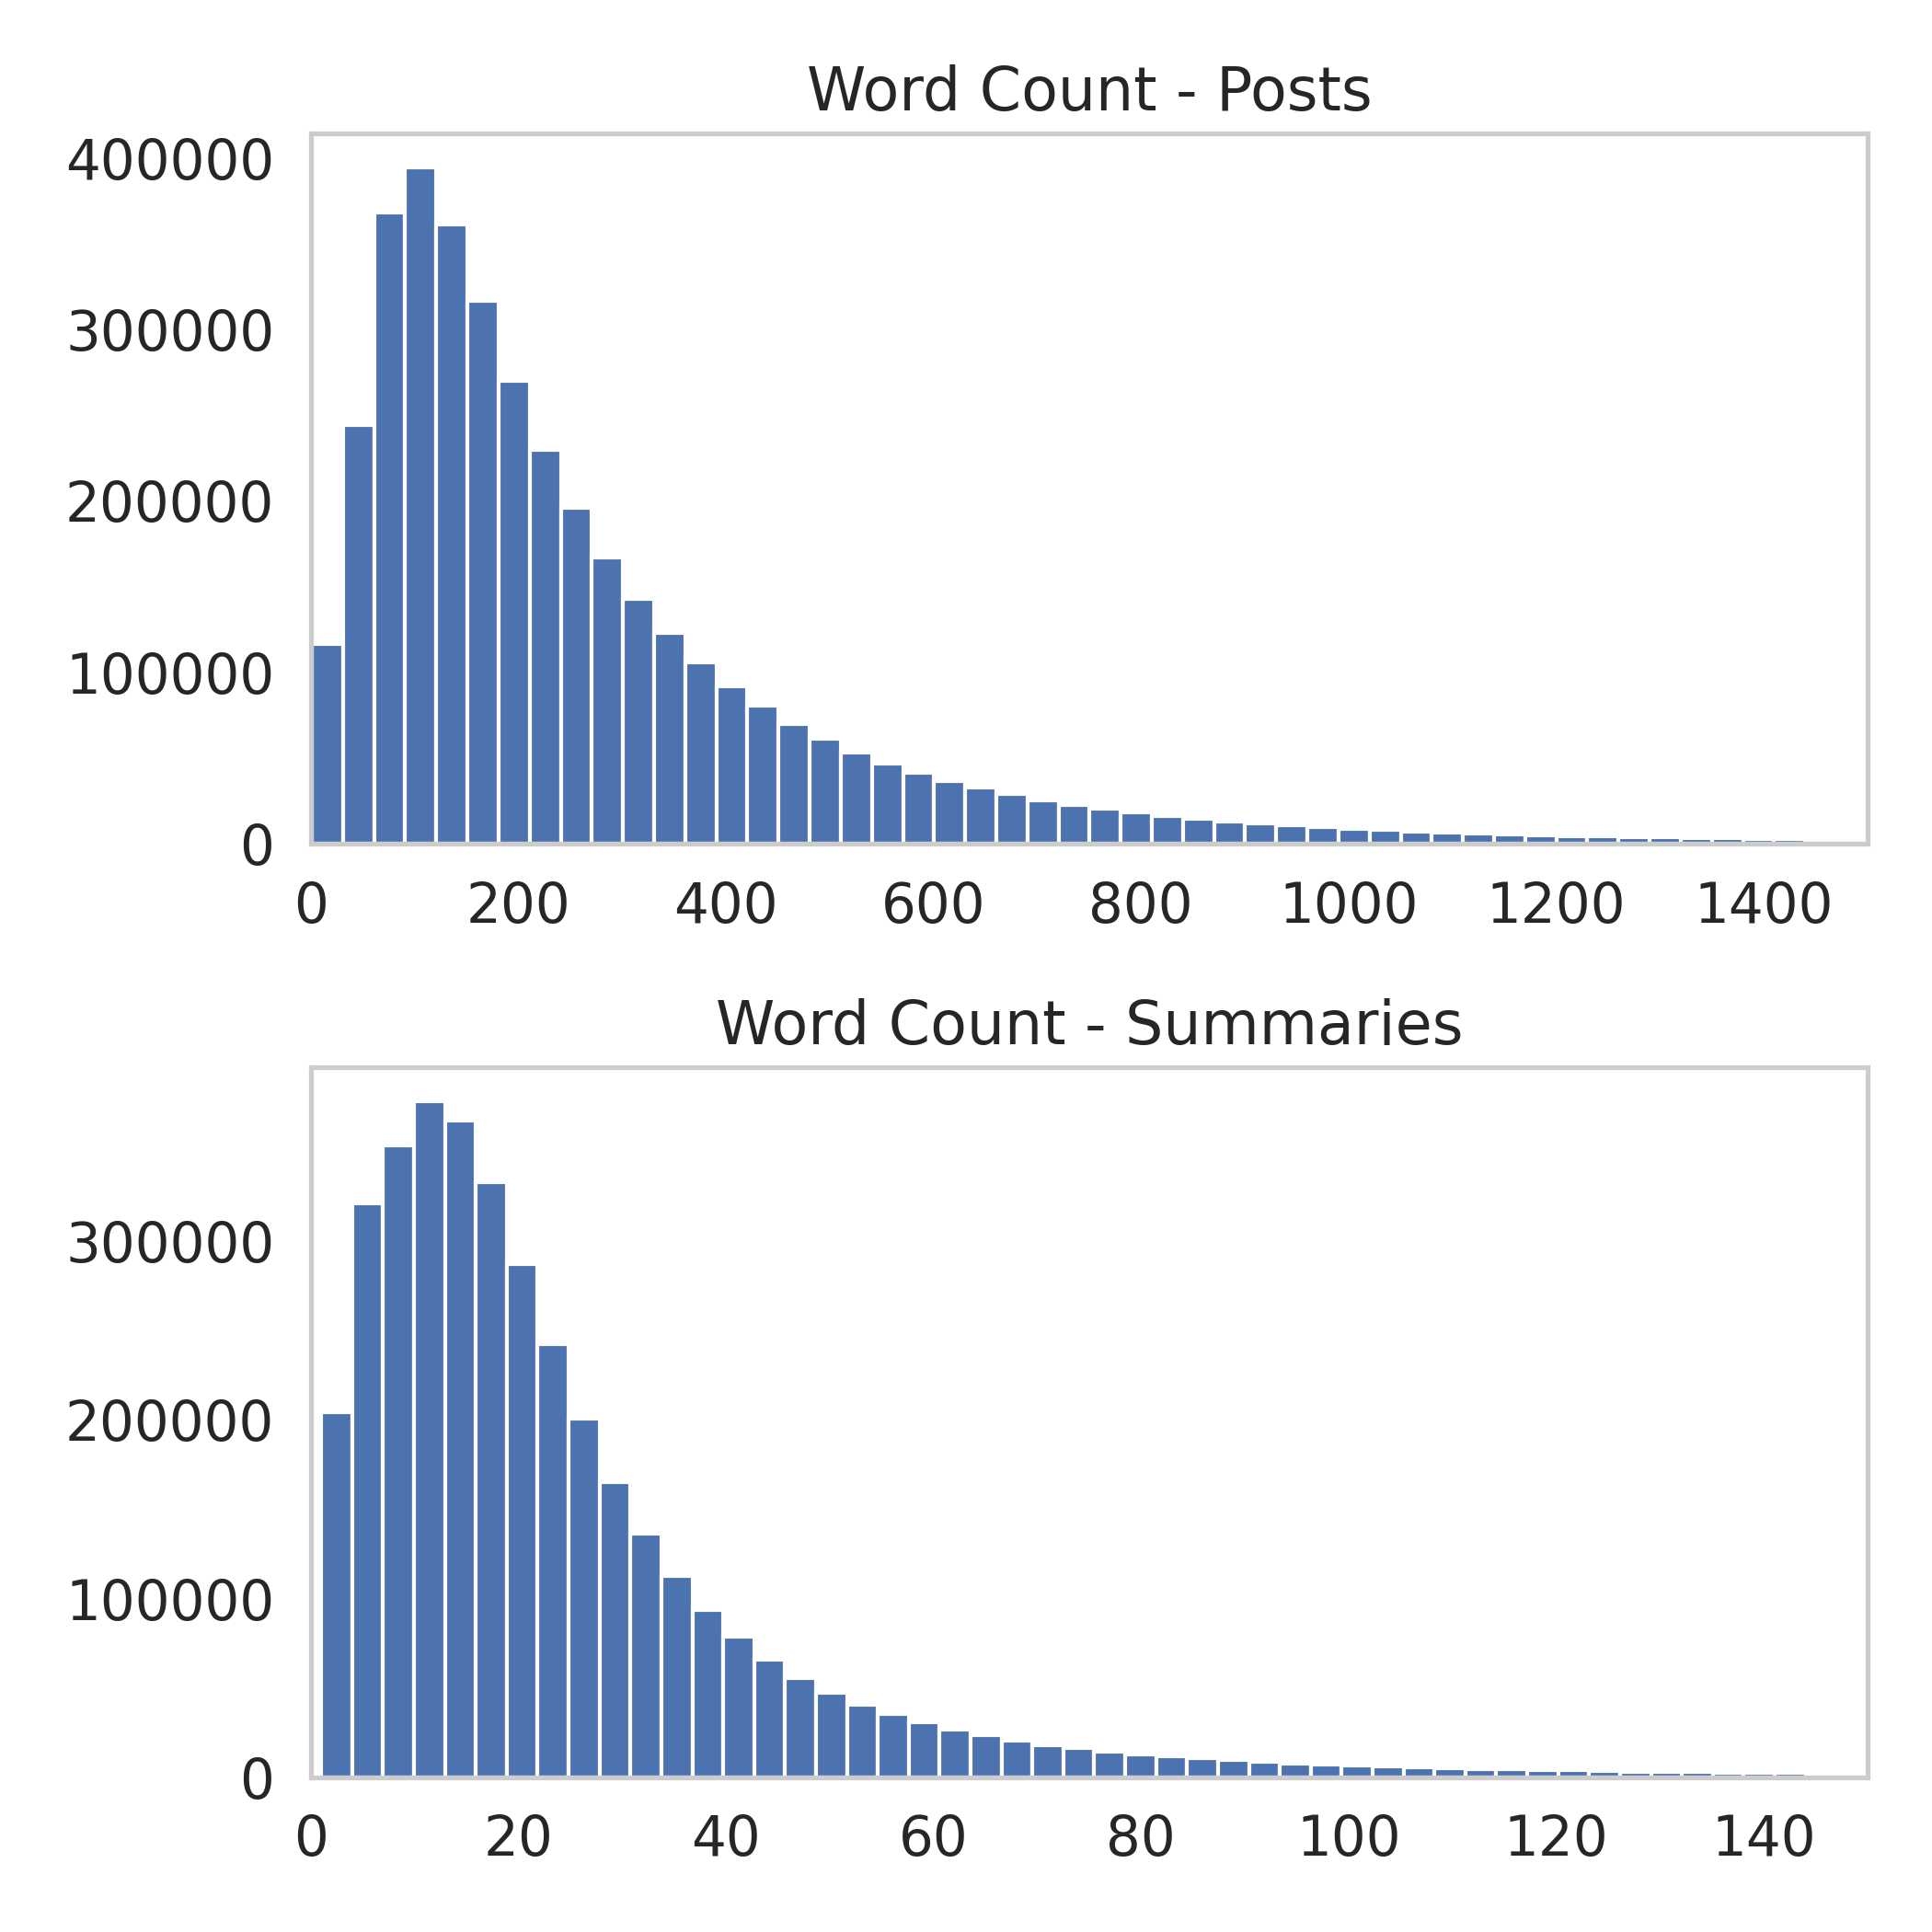
\includegraphics[width=.95\linewidth]{word_counts.png}
  \caption{Word count distributions}
  \label{fig:word_counts}
\end{figure}


Next, we looked into individual observations in the data to understand the data on a more granular level. 
Some Reddit posts and summaries would nonsensically repeat the same word over and over, or just contain one word. 
With this in mind, we decided to filter down the dataset so it would only include posts with word counts between 20 - 1000 and with at least 10 unique words. 
In addition, each summary would only include between 2 - 100 total words and at least 2 unique words. 
With these filters in place, about 300,000 records were removed from our dataset and we were able to deal with higher quality data. 

\subsection{Subreddit Genres}

Each post in our dataset included a subreddit, which conveniently created a category for us. 
We decided to use these categories to our advantage and create segmented NLP models. 
Because there were over 28,000 distinct subreddits in our dataset, it would be unreasonable to build separate NLP models for every distinct subreddit. 
Thus, we sought to group these subreddits into more general genre categories. 

We considered creating a separate NLP model or use unsupervised learning techniques to systematically cluster the subreddits into similar categories, 
but doing so was outside of the scope of what we were seeking to learn through this project. 
Thus, we ended up grouping the subreddits into genres by hand, making sure to categorize the most popular subreddits and create somewhat similar counts in each genre. 
In the end, we grouped the data into 4 distinct subreddit genres: advice/story, gaming, media/lifestyle/sports, and other. 
The counts for each subreddit genre can be found in table 1.

\begin{table}[h]
  \centering
  \begin{tabular}{lrlll}
  \hline \textbf{Subreddit Genre} & \textbf{Post Count}\\ \hline
  Advice/Story & 1409813 \\
  Gaming & 501041 \\
  Media/Liftstyle/Sports & 455228 \\
  Other & 1184045 \\
  \hline
  \end{tabular}
  \caption{\label{subreddit_counts} Subreddit Genres}
\end{table}


\subsection{Modeling}

Sequence to sequence based transformer architectures have proven to achieve state-of-the-art performance on the task of abstractive summarization.
In the original BART paper, the authors explain how BART performs particularly well at text generation as well as for comprehension tasks (Lewis et al., 2019). 
Additionally, recent research has shown that by providing much more data to fine tune the BERT encoder, 
BART achieves state-of-the-art performance on abstractive summarization tasks (Aghajanyan et al., 2020). 

We also explored using Pegasus to generate our summaries. 
Without fine tuning, both Pegasus and BART generated fluent abstractive summaries on our training data. 
Because of BART's strong performance in related research and the ease of use, we decided BART would be a good fit to fine tune on our Reddit data. 
In particular, we used a BART model that was pretrained on both XSUM and CNN/DM datasets because it provided fluent summaries on our data without initial fine tuning. 

After we began training BART models on our dataset and generating summaries, we quickly realized that the scale of our dataset would be a problem. 
We frequently ran out of memory, or would exhaust compute times during training and inference. 
Thus, we decided to downsample our large dataset to a more reasonable scale for our project. 
From our cleaned dataset, we randomly sampled 17,000 observations from each of our 4 subreddit groups,
of which 1,000 would be used for validation and 1,000 would be used for testing. 
Table 2 shows the final observations counts we used in our analysis in each respective subreddit genre, including average word counts. 

\begin{table*}
  \centering
  \begin{tabular}{lccc}
  \hline \textbf{Dataset} & \textbf{\# docs (train/val/test)} & \textbf{avg. post length} & \textbf{avg. summary legnth} \\ \hline
  %\textbf{} & textbf{} & \multicolumn{words}{sentences} & \multicolumn{words}{sentences} \\
  Overall & 60,000/4,000/4,000  & 235 & 22 \\
  Advice/Story & 15,000/1,000/1,000 & 278 & 23 \\
  Gaming & 15,000/1,000/1,000 & 211 & 23 \\
  Media/Lifestyle/Sports & 15,000/1,000/1,000 & 210 & 21 \\
  Other & 15,000/1,000/1,000 & 240 & 23 \\
  \hline
  \end{tabular}
  \caption{\label{final_counts} Comparison of summarization datasets with respect to overall corpus size, size of training, validation, and
  test set, and average post and summary word length}
\end{table*}

Because the Reddit posts had different content in the subreddit genres, 
we hypothesized that we could maximize ROUGE score by training separate BART models on each genre.
Thus, we trained four independent BART models on each of the 15,000 training observations in each subreddit genre. 
Then separately, we trained a full BART model on all of our 60,000 training observations to compare performance. 
Our analysis compares ROUGE scores from the following three models:

\begin{enumerate}
  \item BART Baseline: Pretrained on XSUM and CNN/DM without any fine tuning
  \item BART Full: Fine tuned on our entire Reddit dataset irrespective of subreddit
  \item BART Subreddit Split: Four separate models fine tuned on each of our four subreddit genre categories
\end{enumerate}

For each BART model, we tokenized the Reddit posts to a maximum of 1024 tokens, and the summaries to a maximum of 128 tokens. 
Doing so would adequately tokenize the entire text for over 97\% of our data, and avoid overburdening our BART model with tokens being too long. 

Through this training process, we learned the hard way the importance of checkpointing the model progress often. 
Model training would sometimes crash or exhaust memory resources, and it was helpful to continue training from a checkpoint. 

\section{Results and discussion}

\subsection{Results}

After the fine tuning was completed, we used each of our three BART modeling approaches to generate abstractive summaries on 
our held out 4,000 test observations. Because over 90\% of our target summaries were shorter than 60 words, we decided to 
restrict our BART models to generate summaries with a maximum of 60 words. 

Our primary metric for evaluation was ROUGE. 
Not only is ROUGE the primary metric used to measure performance in related research, 
but the recall based approach was fitting for our analysis because we were most interested in having our summaries adequately capture the important words in the summary. 
Additionally, our 60 word maximum restriction provided a guardrail against the model having a terribly low precision.

To benchmark our model performance, we found the results of other researchers who explored the same Reddit dataset (Syed et al. 2018). 
The researchers report several summarization models they used in their research with a model they call "tldr-bottom-up" having the highest ROUGE score. 
The report does not provide a description of the nature of their "tldr-bottom-up" model. 
Because we used a much smaller sample of the dataset, the results aren't exactly comparable, 
but it provides a reference point to judge our model's performance. 

The resulting ROUGE scores for each of our BART models, as well as the performance from Syed et al., can be found in table 3.

\begin{table}[h]
  \centering
  \begin{tabular}{lrlll}
  \hline \textbf{Test Set and Model} & \textbf{R-1} & \textbf{R-2} & \textbf{R-L} \\ \hline

  \multicolumn{4}{ l }{\emph{Genre: Advice/Story}} \\
  BART Baseline & 16.8 & 2.5 & 13.5 \\
  BART Full & \textbf{20.2} & \textbf{5.9} & \textbf{16.7} \\
  BART Subreddit Split & 20.0 & 5.7 & 16.4 \\
  \hline
  
  \multicolumn{4}{ l }{\emph{Genre: Gaming}} \\
  BART Baseline & 15.3 & 1.9 & 12.0 \\
  BART Full & \textbf{16.5} & \textbf{4.1} & \textbf{13.5} \\
  BART Subreddit Split & 15.5 & 3.7 & 12.7 \\
  \hline

  \multicolumn{4}{ l }{\emph{Genre: Media/Lifestyle/Sports}} \\
  BART Baseline & \textbf{14.8} & 2.1 & 12.1 \\
  BART Full & 14.3 & \textbf{3.5} & \textbf{12.2} \\
  BART Subreddit Split & 14.0 & 3.1 & 11.8 \\
  \hline

  \multicolumn{4}{ l }{\emph{Genre: Other}} \\
  BART Baseline & 14.9 & 2.0 & 12.1 \\
  BART Full & 16.6 & 4.0 & 13.9 \\
  BART Subreddit Split & \textbf{16.8} & \textbf{4.3} & \textbf{14.1} \\
  \hline

  \multicolumn{4}{ l }{\emph{Benchmark (Syed et al.)}} \\
  tldr-bottom-up & 20 & 4 & 15 \\
  \hline

  \end{tabular}
  \caption{\label{test_performance} ROUGE-1,2, and L scores for the generated summaries}
\end{table}

According to ROUGE metrics, the full BART model generally outperformed the others. 
In terms of ROUGE-1, the benchmark "tldr-bottom-up" model generally performs best. 
But our BART Full model often has the highest ROUGE-2 and ROUGE-L scores. 
A key learning for us here is that in the case of our Reddit subset dataset, 
fine tuning on more data seems to be better than fine tuning on more specialized but less data. 

\subsection{Error Analysis}

Next, we dug into the observations that had the lowest ROUGE scores at inference time to study where our models went wrong. 
We were surprised to find that quite often, we felt our BART models produced TL;DR summaries that were even better than the true target summaries. 
It seems the true user-created summaries were sometimes trying to be funny or didn't actually summarize the content faithfully. 
Whereas our BART models seemed to do a better job in these cases. 
As an example, one post was a long story about a user's addiction to cannabis and his desire to abstain from smoking for a month. 
We've pasted the summaries below to show how we feel the BART summary does a better job at providing a more fluent and faithful summary than the true summary. 

\begin{itemize}
  \item True summary: Stay sober through October.
  \item BART Full summary: I'm taking a month off from smoking weed to prove to myself that it's not an issue.
\end{itemize}

On the other hand, there were some situations where our BART model clearly couldn't summarize the content very well. 
Sometimes the BART models would just return the first few words of the content as its summary. 
Other times the BART models would regurgitate important words from the content, but didn't actually provide a sensical summary. 
We hypothesize that our BART models might perform better in some of these situations if we had more computing power to train the model on more observations. 

\subsection{Manual Summary Analysis}

Finally, as an additional benchmark for our models, we decided to manually generate summaries ourselves. 
We wrote 100 summaries, with 25 in each subreddit genre, and computed ROUGE scores on them for comparison. 
While we recognize the small sample size we are using could be a noisy estimate of the total dataset, 
this gives an interesting benchmark and insight into how well we'd hope our BART model could perform.
For simplicity, we only compare the full BART model metrics to our manual summaries in table 4. 

\begin{table}[h]
  \centering
  \begin{tabular}{lrlll}
  \hline \textbf{Summarization Source} & \textbf{R-1} & \textbf{R-2} & \textbf{R-L} \\ \hline

  \multicolumn{4}{ l }{\emph{Genre: Advice/Story}} \\
  BART Full & 24.9 & 7.8 & 20.2 \\
  Manual Summary & 26.4 & 11.3 & 22.7 \\
  \hline
  
  \multicolumn{4}{ l }{\emph{Genre: Gaming}} \\
  BART Full & 19.6 & 7.7 & 17.8 \\
  Manual Summary & 19.5 & 4.8 & 15.5 \\
  \hline

  \multicolumn{4}{ l }{\emph{Genre: Media/Lifestyle/Sports}} \\
  BART Full & 13.1 & 1.2 & 11.1 \\
  Manual Summary & 17.9 & 3.3 & 14.8 \\
  \hline

  \multicolumn{4}{ l }{\emph{Genre: Other}} \\
  BART Full & 13.0 & 4.5 & 11.8 \\
  Manual Summary & 21.1 & 6.1 & 17.3 \\
  \hline

  \end{tabular}
  \caption{\label{manual_summary} Manual Summary Comparisons}
\end{table}

In most cases, our manually generated summaries outperform the BART model by several ROUGE points. 
However, while manually generating the summaries, we found it particularly difficult to summarize the gamming subreddits because they often contained a lot of jargon that we didn't understand. 
It was interesting to us that the BART model actually outperformed our manually generated summaries for the gaming subreddit genre. 

\section{Conclusion}
We find that a BART model trained on a larger generalized social media dataset produces higher ROUGE scores than an equivalent model trained on a smaller genre specific dataset. This generalized BART model achieves similar performance to the “tldr-bottom-up” model from prior research. For next steps, it may be interesting to explore if the size of the genre specific dataset was increased if the same pattern holds true.

\section*{References}
 \noindent Armen Aghajanyan; Akshat Shrivastava; Anchit Gupta; Naman Goyal; Luke Zettlemoyer; Sonal Gupta. 2021. Better Fine-Tuning by Reducing Representational Collapse. \emph{ArXiv: 2008.03156}
 \bigbreak
\noindent Chin-Yew Lin. 2004. Rouge: A package for auto-
matic evaluation of summaries. \emph{Text Summarization
Branches Out.}
\bigbreak
\noindent Mike Lewis; Yinhan Liu; Naman Goyal; Marjan Ghazvininejad; Abdelrahman Mohamed; Omer Levy; Veselin Stoyanov; Luke Zettlemoyer. 2020. BART: Denoising Sequence-to-Sequence Pre-training for Natural Language Generation, Translation, and Comprehension. \emph{ArXiv: 1910.13461}
\bigbreak
\noindent Shahbaz Syed; Michael Völske; Nedim Lipka; Benno Stein; Hinrich Schütze; Martin Potthast. 2019. Towards summarization for social media-results of the tl;dr
challenge. \emph{In Proceedings of the 12th International Conference on Natural Language Generation, Tokyo, Japan, 29 October–1
November 2019; pp. 523–528}
\bigbreak
\noindent Yiran Chen; Pengfei Liu; Ming Zhong; Zi-Yi Dou; Danquing Wang; Xipeng Qiu; Xuanjing Huang. 2020. CDEvalSumm: An empirical study of cross-dataset evaluation
for neural summarization systems. \emph{"Findings of the Association for Computational Linguistics: EMNLP 2020"}

\end{document}

